\begin{tikzpicture}
\node [rectangle, inner sep=0.5pt, draw, thick, draw=color1] (target) {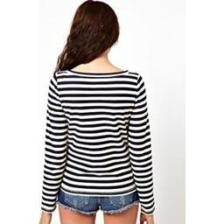
\includegraphics[width=2cm] {../thesis/images/adv/target}};

\node [above=of target, yshift=-1cm, color1, font=\small] {Target image};

\node [below=1.25cm of target, rectangle, inner sep=0.5pt, draw, thick, draw=color3] (attack) {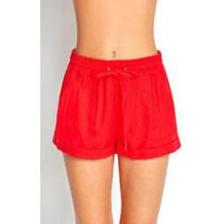
\includegraphics[width=2cm] {../thesis/images/adv/original}};
\node [above=of attack, yshift=-1cm, color3, font=\small] {Attack image};

\node [right=of target, trapezium, trapezium angle=70, minimum width=1.5cm, shape border rotate=270, draw=color2, fill=color2!50, thick] (conv1) {\tiny $CONV$};
\node [right=of attack, trapezium, trapezium angle=70, minimum width=1.5cm, shape border rotate=270, draw=color2, fill=color2!50, thick] (conv2) {\tiny $CONV$};

\node [right=of conv1, rectangle, minimum height=2.5cm, minimum width=0.65cm, draw=color1, fill=color1!50, thick, align=center] (feat1) {$x_t$};
\node [right=of conv2, rectangle, minimum height=2.5cm, minimum width=0.65cm, draw=color3, fill=color3!50, thick, align=center] (feat2) {$x_a$};

\node [above=of feat1, yshift=-1cm, color0!25!black, font=\small] {Feature vectors};

\node [right=of $(feat1)!0.5!(feat2)$, rectangle, rounded corners, minimum height=0.8cm, draw, draw=color4, fill=color4!50, thick] (simi) {\scriptsize$sim(x_t, x_a)$};
\node [right=of simi, color4, align=center, font=\small] (out) {$dist$};

\path [<->, draw, color2, thick] (conv1) to node[right, 
align=left, font=\scriptsize]{Shared\\ weights} (conv2) {};
\path [->, draw, color1!75] (target) to (conv1) {};
\path [->, draw, color3!75] (attack.east) +(0,0.5em) coordinate (attackIn) to (conv2.west |- attackIn) {};
\path [->, draw, color3, densely dashed, very thick] (conv2.west) +(0,-0.5em) coordinate (convGrad) to (attack.east |- convGrad) {};

\path [->, draw, color1!75] (conv1) to (feat1) {};
\path [->, draw, color3!75] (conv2.east) +(0,0.5em) coordinate (convOut) to (feat2.west |- convOut) {};
\path [->, draw, color3, densely dashed, very thick] (feat2.west) +(0,-0.5em) coordinate (featGradOut) to (conv2.east |- featGradOut) {};

\path [->, draw, color1!75, bend left] (feat1) to (simi.north) {};
\path (simi.south) +(-0.5em,0) coordinate (simiIn) {};
\path [->, draw, color3!75, bend right] (feat2.east) +(0,0.5em) to (simiIn) {};
\path (feat2.east) +(0,-0.5em) coordinate (featGradIn) {};
\path [->, draw, color3, densely dashed, very thick, bend left] (simi.south) +(0.5em,0) to node[right=1em, font=\small] {$gradients$} (featGradIn) {};
\path [->, draw, color4] (simi) to (out) {};

\end{tikzpicture}